\begin{figure}[t]
    \centering
    \hspace*{\fill}
  \subfloat[\label{fig:merrer-a}]{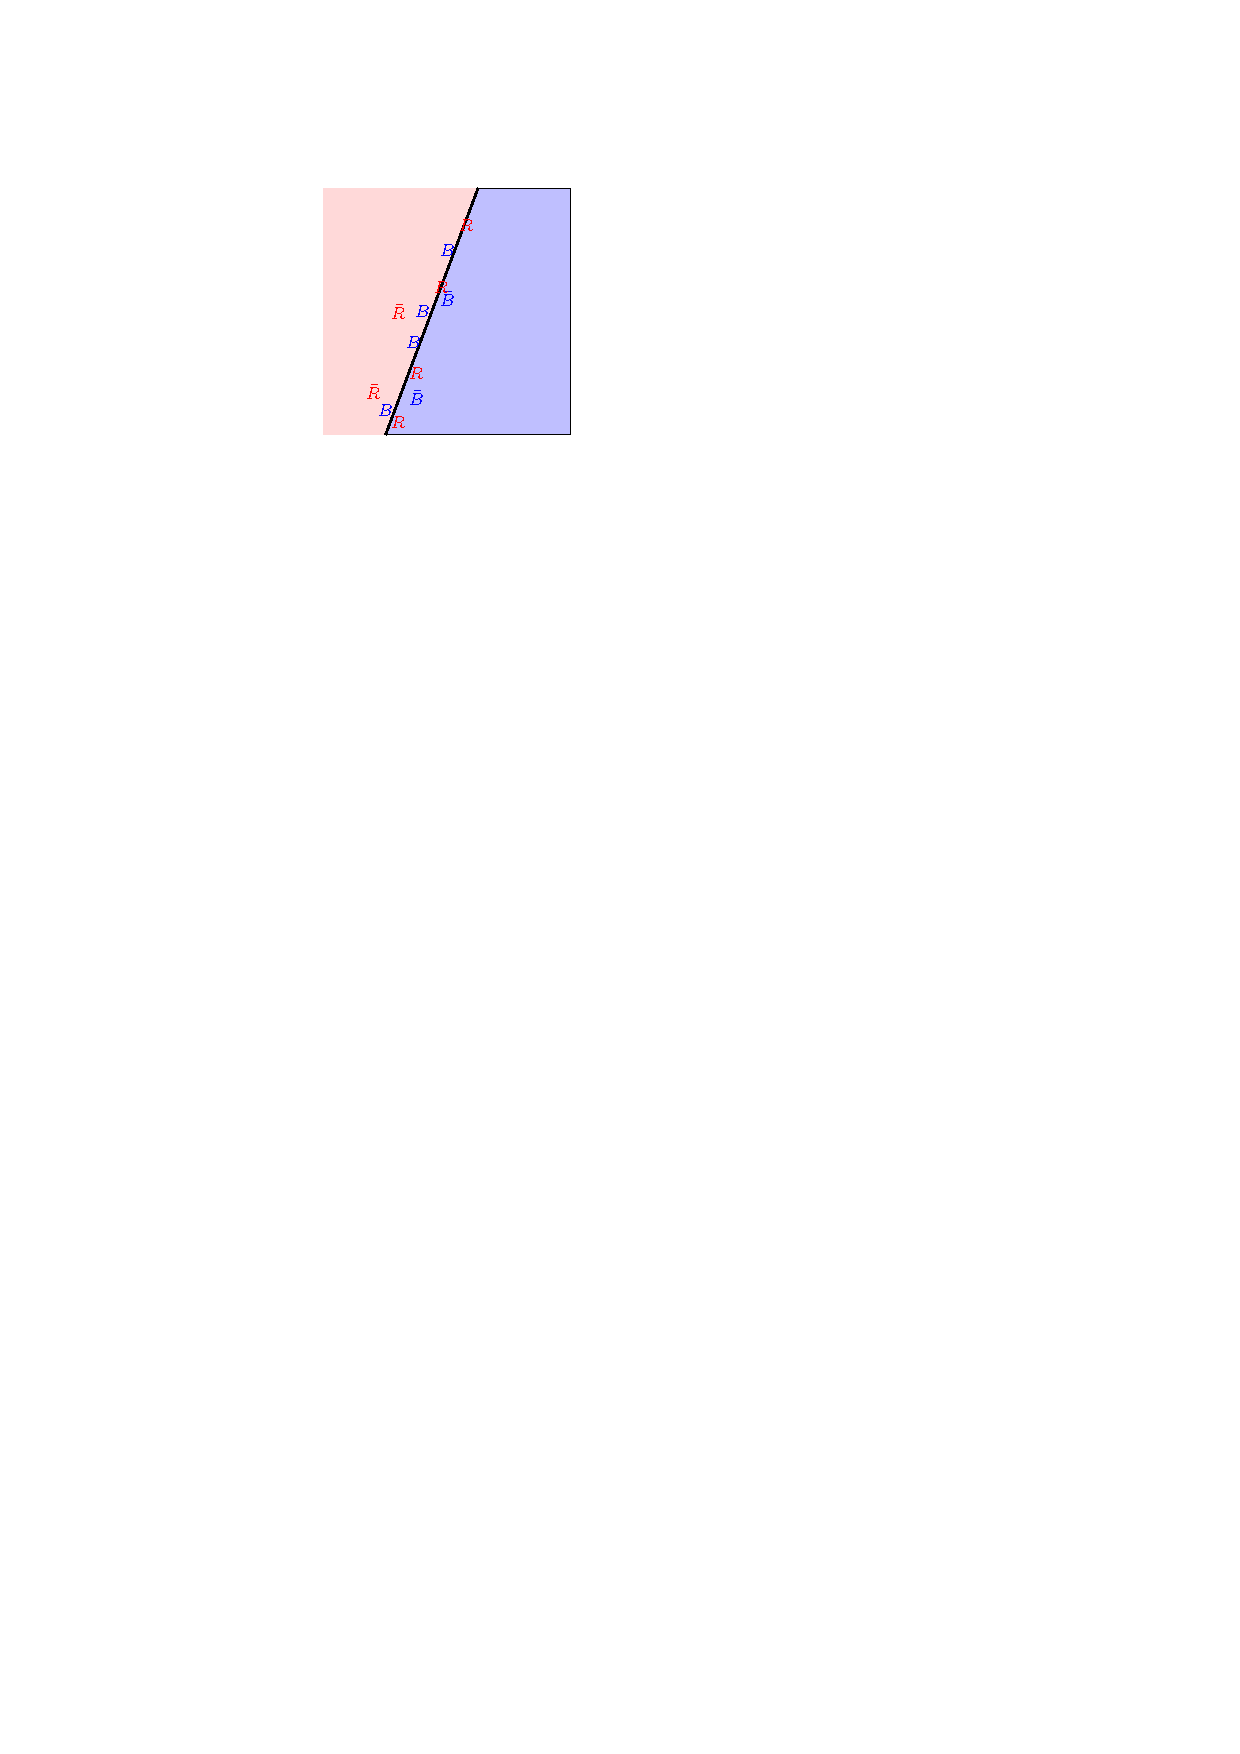
\includegraphics[width = 0.2 \textwidth]{images/frontier/Merrer1.pdf}}
    \quad
  \subfloat[\label{fig:merrer-b}]{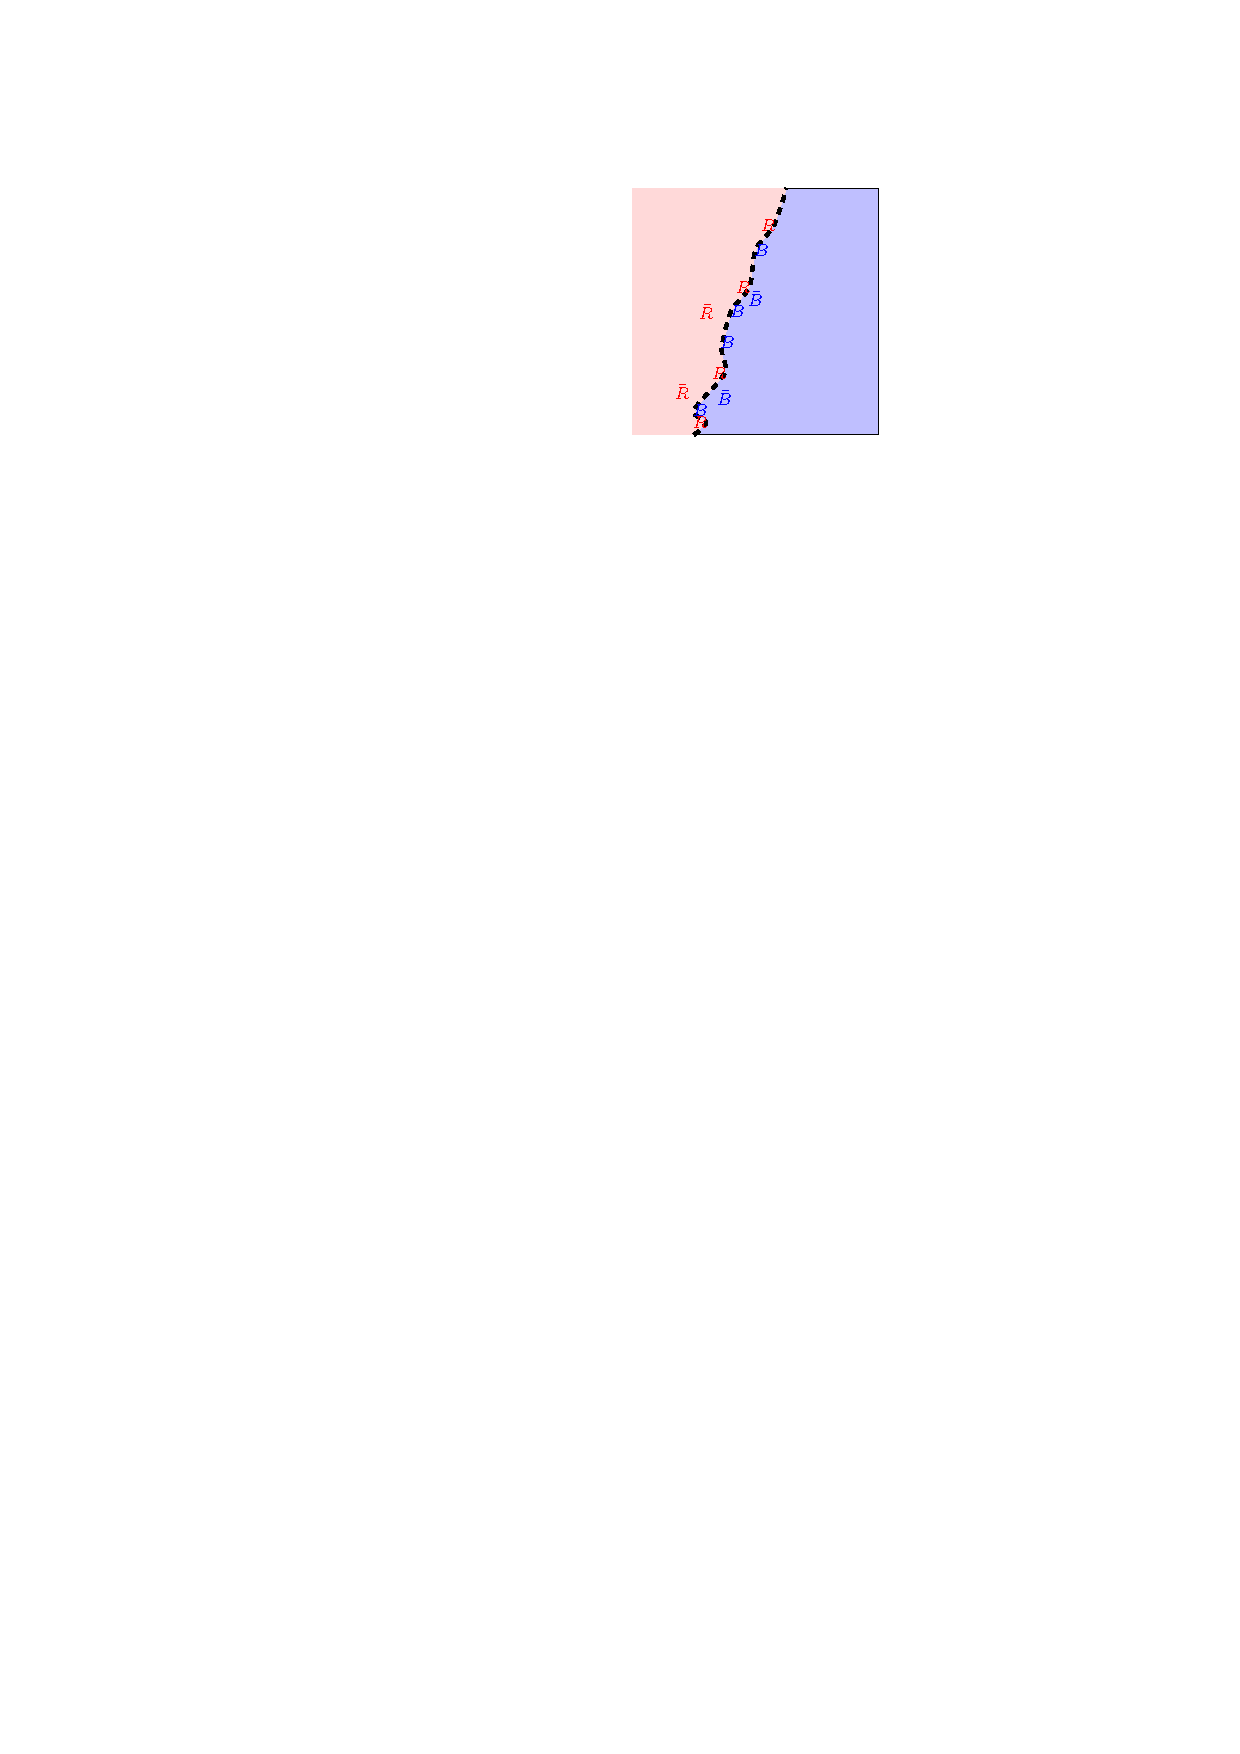
\includegraphics[width = 0.2 \textwidth]{images/frontier/Merrer2.pdf}}
    \hspace*{\fill}
    \caption{(a) The data points are divided into "true adversaries" ($R$ and $B$) and "false adversaries" ($\bar{R}$ and $\bar{B}$). The label for the true adversaries is changed, the label for the false adversaries stays unchanged. (b) After fine-tuning the decision boundary changes. \cite{merrer_adversarial_2019}}
    \label{fig:merrer}
\end{figure}